

\tikzset{every picture/.style={line width=0.75pt}} %set default line width to 0.75pt        

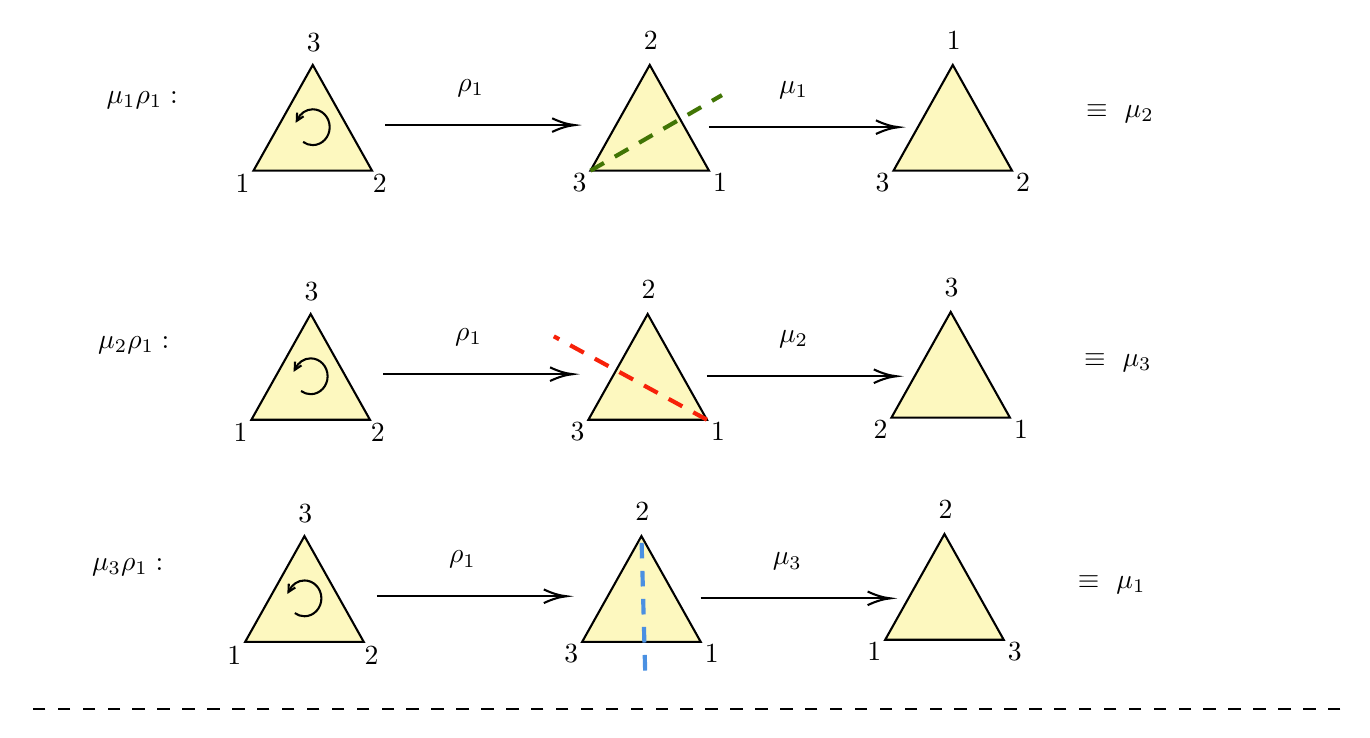
\begin{tikzpicture}[x=0.75pt,y=0.75pt,yscale=-1,xscale=1]
%uncomment if require: \path (0,350); %set diagram left start at 0, and has height of 350

%Shape: Triangle [id:dp18279766660658403] 
\draw  [fill={rgb, 255:red, 250; green, 238; blue, 106 }  ,fill opacity=0.43 ] (141.85,151.75) -- (170.41,202.69) -- (113.29,202.69) -- cycle ;
%Shape: Triangle [id:dp4197310425493971] 
\draw  [fill={rgb, 255:red, 250; green, 238; blue, 106 }  ,fill opacity=0.43 ] (304.21,151.75) -- (332.76,202.69) -- (275.65,202.69) -- cycle ;

%Straight Lines [id:da930520097755943] 
\draw    (176.75,180.73) -- (266.12,180.73) ;
\draw [shift={(268.12,180.73)}, rotate = 180] [color={rgb, 255:red, 0; green, 0; blue, 0 }  ][line width=0.75]    (10.93,-3.29) .. controls (6.95,-1.4) and (3.31,-0.3) .. (0,0) .. controls (3.31,0.3) and (6.95,1.4) .. (10.93,3.29)   ;
%Shape: Arc [id:dp215844960607804] 
\draw  [draw opacity=0] (134.49,178.01) .. controls (135.81,175.11) and (138.61,173.11) .. (141.85,173.11) .. controls (146.36,173.11) and (150.01,176.97) .. (150.01,181.74) .. controls (150.01,186.5) and (146.36,190.37) .. (141.85,190.37) .. controls (140.13,190.37) and (138.53,189.8) .. (137.21,188.84) -- (141.85,181.74) -- cycle ; \draw   (134.49,178.01) .. controls (135.81,175.11) and (138.61,173.11) .. (141.85,173.11) .. controls (146.36,173.11) and (150.01,176.97) .. (150.01,181.74) .. controls (150.01,186.5) and (146.36,190.37) .. (141.85,190.37) .. controls (140.13,190.37) and (138.53,189.8) .. (137.21,188.84) ;  
\draw   (137.43,176.51) -- (134.15,178.67) -- (134.31,174.69) ;

%Straight Lines [id:da5632790371547318] 
\draw [color={rgb, 255:red, 247; green, 33; blue, 9 }  ,draw opacity=1 ][line width=1.5]  [dash pattern={on 5.63pt off 4.5pt}]  (332.76,202.69) -- (259,162.5) ;
%Shape: Triangle [id:dp6887834214805665] 
\draw  [fill={rgb, 255:red, 250; green, 238; blue, 106 }  ,fill opacity=0.43 ] (450.21,150.75) -- (478.76,201.69) -- (421.65,201.69) -- cycle ;

%Straight Lines [id:da8273926927450299] 
\draw    (332.75,181.73) -- (422.12,181.73) ;
\draw [shift={(424.12,181.73)}, rotate = 180] [color={rgb, 255:red, 0; green, 0; blue, 0 }  ][line width=0.75]    (10.93,-3.29) .. controls (6.95,-1.4) and (3.31,-0.3) .. (0,0) .. controls (3.31,0.3) and (6.95,1.4) .. (10.93,3.29)   ;
%Shape: Triangle [id:dp13836286231856076] 
\draw  [fill={rgb, 255:red, 250; green, 238; blue, 106 }  ,fill opacity=0.43 ] (142.85,31.75) -- (171.41,82.69) -- (114.29,82.69) -- cycle ;
%Shape: Triangle [id:dp9253244528119978] 
\draw  [fill={rgb, 255:red, 250; green, 238; blue, 106 }  ,fill opacity=0.43 ] (305.21,31.75) -- (333.76,82.69) -- (276.65,82.69) -- cycle ;

%Straight Lines [id:da23996092927188062] 
\draw    (177.75,60.73) -- (267.12,60.73) ;
\draw [shift={(269.12,60.73)}, rotate = 180] [color={rgb, 255:red, 0; green, 0; blue, 0 }  ][line width=0.75]    (10.93,-3.29) .. controls (6.95,-1.4) and (3.31,-0.3) .. (0,0) .. controls (3.31,0.3) and (6.95,1.4) .. (10.93,3.29)   ;
%Shape: Arc [id:dp8896128197930823] 
\draw  [draw opacity=0] (135.49,58.01) .. controls (136.81,55.11) and (139.61,53.11) .. (142.85,53.11) .. controls (147.36,53.11) and (151.01,56.97) .. (151.01,61.74) .. controls (151.01,66.5) and (147.36,70.37) .. (142.85,70.37) .. controls (141.13,70.37) and (139.53,69.8) .. (138.21,68.84) -- (142.85,61.74) -- cycle ; \draw   (135.49,58.01) .. controls (136.81,55.11) and (139.61,53.11) .. (142.85,53.11) .. controls (147.36,53.11) and (151.01,56.97) .. (151.01,61.74) .. controls (151.01,66.5) and (147.36,70.37) .. (142.85,70.37) .. controls (141.13,70.37) and (139.53,69.8) .. (138.21,68.84) ;  
\draw   (138.43,56.51) -- (135.15,58.67) -- (135.31,54.69) ;

%Shape: Triangle [id:dp795571423848466] 
\draw  [fill={rgb, 255:red, 250; green, 238; blue, 106 }  ,fill opacity=0.43 ] (451.21,31.75) -- (479.76,82.69) -- (422.65,82.69) -- cycle ;

%Straight Lines [id:da9572482179097236] 
\draw    (333.75,61.73) -- (423.12,61.73) ;
\draw [shift={(425.12,61.73)}, rotate = 180] [color={rgb, 255:red, 0; green, 0; blue, 0 }  ][line width=0.75]    (10.93,-3.29) .. controls (6.95,-1.4) and (3.31,-0.3) .. (0,0) .. controls (3.31,0.3) and (6.95,1.4) .. (10.93,3.29)   ;
%Straight Lines [id:da20730078002652064] 
\draw [color={rgb, 255:red, 65; green, 117; blue, 5 }  ,draw opacity=1 ][line width=1.5]  [dash pattern={on 5.63pt off 4.5pt}]  (276.65,82.69) -- (340,46.3) ;
%Shape: Triangle [id:dp26218350538367785] 
\draw  [fill={rgb, 255:red, 250; green, 238; blue, 106 }  ,fill opacity=0.43 ] (138.85,258.75) -- (167.41,309.69) -- (110.29,309.69) -- cycle ;
%Shape: Triangle [id:dp7257387830462504] 
\draw  [fill={rgb, 255:red, 250; green, 238; blue, 106 }  ,fill opacity=0.43 ] (301.21,258.75) -- (329.76,309.69) -- (272.65,309.69) -- cycle ;

%Straight Lines [id:da43043420907131935] 
\draw    (173.75,287.73) -- (263.12,287.73) ;
\draw [shift={(265.12,287.73)}, rotate = 180] [color={rgb, 255:red, 0; green, 0; blue, 0 }  ][line width=0.75]    (10.93,-3.29) .. controls (6.95,-1.4) and (3.31,-0.3) .. (0,0) .. controls (3.31,0.3) and (6.95,1.4) .. (10.93,3.29)   ;
%Shape: Arc [id:dp2345241317556913] 
\draw  [draw opacity=0] (131.49,285.01) .. controls (132.81,282.11) and (135.61,280.11) .. (138.85,280.11) .. controls (143.36,280.11) and (147.01,283.97) .. (147.01,288.74) .. controls (147.01,293.5) and (143.36,297.37) .. (138.85,297.37) .. controls (137.13,297.37) and (135.53,296.8) .. (134.21,295.84) -- (138.85,288.74) -- cycle ; \draw   (131.49,285.01) .. controls (132.81,282.11) and (135.61,280.11) .. (138.85,280.11) .. controls (143.36,280.11) and (147.01,283.97) .. (147.01,288.74) .. controls (147.01,293.5) and (143.36,297.37) .. (138.85,297.37) .. controls (137.13,297.37) and (135.53,296.8) .. (134.21,295.84) ;  
\draw   (134.43,283.51) -- (131.15,285.67) -- (131.31,281.69) ;

%Shape: Triangle [id:dp1407114381804121] 
\draw  [fill={rgb, 255:red, 250; green, 238; blue, 106 }  ,fill opacity=0.43 ] (447.21,257.75) -- (475.76,308.69) -- (418.65,308.69) -- cycle ;

%Straight Lines [id:da39649581628084885] 
\draw    (329.75,288.73) -- (419.12,288.73) ;
\draw [shift={(421.12,288.73)}, rotate = 180] [color={rgb, 255:red, 0; green, 0; blue, 0 }  ][line width=0.75]    (10.93,-3.29) .. controls (6.95,-1.4) and (3.31,-0.3) .. (0,0) .. controls (3.31,0.3) and (6.95,1.4) .. (10.93,3.29)   ;
%Straight Lines [id:da39217256062402506] 
\draw [color={rgb, 255:red, 74; green, 144; blue, 226 }  ,draw opacity=1 ][line width=1.5]  [dash pattern={on 5.63pt off 4.5pt}]  (303,323.52) -- (301.21,258.75) ;
%Straight Lines [id:da04582911895669162] 
\draw  [dash pattern={on 4.5pt off 4.5pt}]  (638,341.9) -- (6,341.9) ;

% Text Node
\draw (103.22,203.31) node [anchor=north west][inner sep=0.75pt]    {$1$};
% Text Node
\draw (169.3,203.31) node [anchor=north west][inner sep=0.75pt]    {$2$};
% Text Node
\draw (137.48,135.11) node [anchor=north west][inner sep=0.75pt]    {$3$};
% Text Node
\draw (299.84,134.29) node [anchor=north west][inner sep=0.75pt]    {$2$};
% Text Node
\draw (333.29,202.49) node [anchor=north west][inner sep=0.75pt]    {$1$};
% Text Node
\draw (265.57,202.49) node [anchor=north west][inner sep=0.75pt]    {$3$};
% Text Node
\draw (210,157.4) node [anchor=north west][inner sep=0.75pt]    {$\rho _{1}$};
% Text Node
\draw (445.84,133.29) node [anchor=north west][inner sep=0.75pt]    {$3$};
% Text Node
\draw (479.29,201.49) node [anchor=north west][inner sep=0.75pt]    {$1$};
% Text Node
\draw (411.57,201.49) node [anchor=north west][inner sep=0.75pt]    {$2$};
% Text Node
\draw (366,158.4) node [anchor=north west][inner sep=0.75pt]    {$\mu _{2}$};
% Text Node
\draw (513,169.4) node [anchor=north west][inner sep=0.75pt]    {$\equiv \ \mu _{3}$};
% Text Node
\draw (104.22,83.31) node [anchor=north west][inner sep=0.75pt]    {$1$};
% Text Node
\draw (170.3,83.31) node [anchor=north west][inner sep=0.75pt]    {$2$};
% Text Node
\draw (138.48,15.11) node [anchor=north west][inner sep=0.75pt]    {$3$};
% Text Node
\draw (211,37.4) node [anchor=north west][inner sep=0.75pt]    {$\rho _{1}$};
% Text Node
\draw (366,38.4) node [anchor=north west][inner sep=0.75pt]    {$\mu _{1}$};
% Text Node
\draw (514,49.4) node [anchor=north west][inner sep=0.75pt]    {$\equiv \ \mu _{2}$};
% Text Node
\draw (446.84,14.29) node [anchor=north west][inner sep=0.75pt]    {$1$};
% Text Node
\draw (480.29,82.49) node [anchor=north west][inner sep=0.75pt]    {$2$};
% Text Node
\draw (412.57,82.49) node [anchor=north west][inner sep=0.75pt]    {$3$};
% Text Node
\draw (300.84,14.29) node [anchor=north west][inner sep=0.75pt]    {$2$};
% Text Node
\draw (334.29,82.49) node [anchor=north west][inner sep=0.75pt]    {$1$};
% Text Node
\draw (266.57,82.49) node [anchor=north west][inner sep=0.75pt]    {$3$};
% Text Node
\draw (42,43.12) node [anchor=north west][inner sep=0.75pt]    {$\mu _{1} \rho _{1} :$};
% Text Node
\draw (38,161.12) node [anchor=north west][inner sep=0.75pt]    {$\mu _{2} \rho _{1} :$};
% Text Node
\draw (100.22,310.31) node [anchor=north west][inner sep=0.75pt]    {$1$};
% Text Node
\draw (166.3,310.31) node [anchor=north west][inner sep=0.75pt]    {$2$};
% Text Node
\draw (134.48,242.11) node [anchor=north west][inner sep=0.75pt]    {$3$};
% Text Node
\draw (207,264.4) node [anchor=north west][inner sep=0.75pt]    {$\rho _{1}$};
% Text Node
\draw (363,265.4) node [anchor=north west][inner sep=0.75pt]    {$\mu _{3}$};
% Text Node
\draw (510,276.4) node [anchor=north west][inner sep=0.75pt]    {$\equiv \ \mu _{1}$};
% Text Node
\draw (35,268.12) node [anchor=north west][inner sep=0.75pt]    {$\mu _{3} \rho _{1} :$};
% Text Node
\draw (442.84,240.29) node [anchor=north west][inner sep=0.75pt]    {$2$};
% Text Node
\draw (476.29,308.49) node [anchor=north west][inner sep=0.75pt]    {$3$};
% Text Node
\draw (408.57,308.49) node [anchor=north west][inner sep=0.75pt]    {$1$};
% Text Node
\draw (296.84,241.29) node [anchor=north west][inner sep=0.75pt]    {$2$};
% Text Node
\draw (330.29,309.49) node [anchor=north west][inner sep=0.75pt]    {$1$};
% Text Node
\draw (262.57,309.49) node [anchor=north west][inner sep=0.75pt]    {$3$};


\end{tikzpicture}
